\documentclass[12pt,a4paper]{article}
\usepackage{mathptmx} % added for time new roman font
\usepackage[left=0.5in,right=0.5in,top=1in,bottom=1in]{geometry}
\usepackage[latin1]{inputenc}
\usepackage{amsmath}
\usepackage{amsfonts}
\usepackage{amssymb}
\usepackage{graphicx}
\usepackage{float}
\usepackage{booktabs}
\usepackage{parskip} % remove all the paragraph indents


\usepackage{setspace}
\usepackage[colorlinks=true]{hyperref}
\usepackage{textcomp} 
\usepackage{multicol} 

\usepackage{mathtools}          %loads amsmath as well added for the piece wise function
\DeclarePairedDelimiter\Floor\lfloor\rfloor
\DeclarePairedDelimiter\Ceil\lceil\rceil

 
\newcounter{NumberInTable}
\newcommand{\LTNUM}{\stepcounter{NumberInTable}{(\theNumberInTable)}}

\newcommand{\Laplace}[1]{\ensuremath{\mathcal{L}{\left[#1\right]}}}
\newcommand{\InvLap}[1]{\ensuremath{\mathcal{L}^{-1}{\left[#1\right]}}}
\renewcommand{\textuparrow}{$\uparrow$}

\begin{document}
	
	\large{}
	
	\title{\vspace{-2cm}Lecture Notes, Topic-4}
	\date{}
	\maketitle
	
	\section*{Review from previous class}
	\begin{enumerate}
		\item Solve the ODE
	\item Obtain an equation for the free response of a system
	\end{enumerate}
	
	\section*{Objectives for today's class}
	\begin{enumerate}
		\item Introduce the concept fo damping
		\item Model viscous damping in a 1 DOF system
	\end{enumerate}
	
	\section*{Lecture}
	
		\subsection*{What is damping?}
		
			The response of a spring-mass system predicts that a system will oscillate indefinitely. However, we know that this is not true from observing real-world solutions. So based on real-world observations and mathematical conveniences, we need to add a term that will remove ``energy'' from the system with time. To do this we introduce the ideal dashpot, modeled with the terms $c \dot{x}$.
			
			\begin{figure}[H]
				\centering
				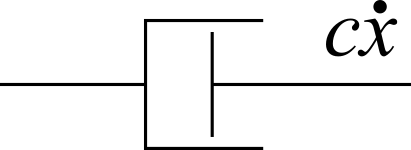
\includegraphics[width=0.3\textwidth]{../../Figures/dashpot.png}
			\end{figure}
			
			A spring forms a physical model of the cause vibration, through its storage and release of energy, a damper forms a physical model for dissipating energy We typically model dampers as viscous dampers, and as such the force is proportional to the velocity of the damper. The damping force $f_c$ has the form 
			\begin{equation}
				f_c = c \dot{x}(t)
			\end{equation}
			
			the constant c, called the damping coefficient, has the units of kg/s.
		
		\subsection*{What does it mean in real life?}
		
			Systems have damping, but not with just physical dampers. Our spring-mass systems are just representations of real-world systems.
			
			
			\begin{figure}[H]
				\centering
				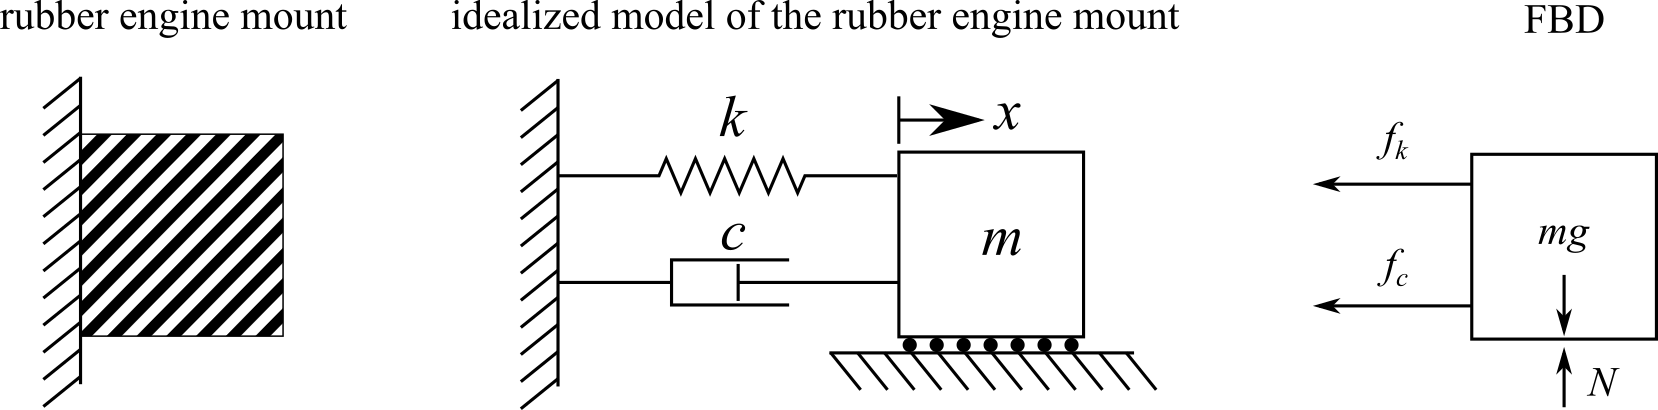
\includegraphics[width=1.0\textwidth]{../../Figures/engine_mount.png}
			\end{figure}

		\subsection*{What does damping look like in terms of displacement vs time}

			\begin{figure}[H]
				\centering
				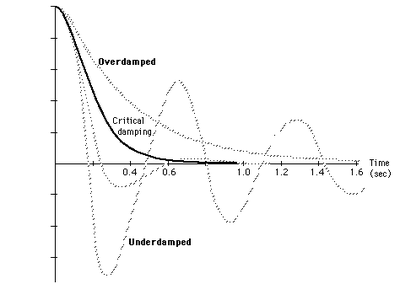
\includegraphics[width=0.6\textwidth]{../../Figures/Damping_plots.png}
			\end{figure}
			
			The key types of damping are:
			\begin{itemize}
			\item \textbf{Undamped} - Oscillates around the equilibrium and does not decay.
			\item \textbf{Under damped} - Oscillates around the equilibrium and slowly decays  and is the most common case.
			\item \textbf{Critically damped} - provides the quickest approach to zero amplitude for a damped oscillator.
			\item \textbf{Overdamped} - Does not pass the equilibrium position and is a simple a decay with no oscillation.
			\end{itemize}
			In this class we are only considering positive damping, mass, and stiffness values.
			
		\subsection*{Solve the EOM with damping?}
					
			Using the FBD for the system, we can conclude that the EOM for this system:
			\begin{figure}[H]
				\centering
				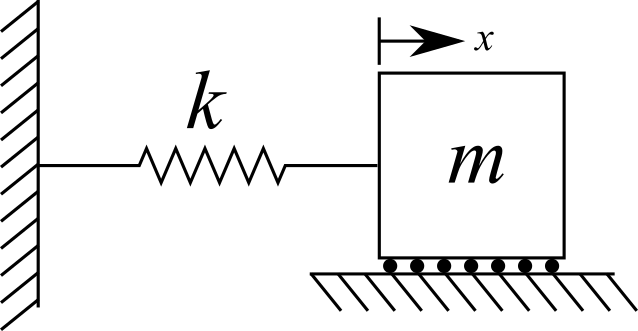
\includegraphics[width=0.3\textwidth]{../../Figures/1-DOF-mass_horizontal.png}
			\end{figure}			
			is:
			\begin{equation}
				m\ddot{x}(t) = - f_c - f_k
			\end{equation}
			Rearranging into standard form and concerting forces into parameters $c$ and $k$ results in:
			\begin{equation}
				m\ddot{x}(t) + c \dot{x}(t) + kx(t) = 0
			\end{equation}
			This system is subject to the same initial conditions as before, $x(0) = x_0$ and $\dot{x}(0) = v_0$. Again, we chose to model it this way for convinces, so let's solve it in a similar manner to the EOM without damping. Again, assume the solution:
			\begin{equation}
				x(t) = ae^{\lambda t}
			\end{equation}
			here, $a$ and $t$ are nonzeros constants that need to be determined.  Using successive differentiation, we get:
			\begin{equation}
				\dot{x}(t) = \lambda ae^{\lambda t}
			\end{equation}
			and 
			\begin{equation}
				\ddot{x}(t) = \lambda^2 ae^{\lambda t}
			\end{equation}
			therefore, $m\ddot{x} + c\dot{x} + kx = 0$ becomes:
			\begin{equation}
				m \lambda^2 ae^{\lambda t}  +c\lambda ae^{\lambda t} + k ae^{\lambda t} = 0
			\end{equation}
			Now we divide by $ae^{\lambda t}$ to obtain the \textbf{characteristic equation}:
			\begin{equation}
				m \lambda^2 + c\lambda + k = 0
			\end{equation}
			We can do this because $ae^{\lambda t}$ is never zero, therefore, we never divide by zero. The quadratic formula gives us:
			\begin{equation}
				\lambda_{1,2} = \frac{-c \pm \sqrt{c^2-4km}}{2m}  = \frac{-c}{2m} \pm \frac{1}{2m}\sqrt{c^2-4km}
			\end{equation}
			Some key points from this equation:
			\begin{itemize}
			\item The $\pm$ tells us there are two solutions to this problem
			\item if $c^2-4km<0$, system is Underdamped, solutions are complex conjugate pairs 
			\item if $c^2-4km=0$, system is critically damped, solutions are equal negative real numbers 
			\item if $c^2-4km>0$, system is Overdamped, solutions are distinct negative real numbers 
			\end{itemize}
			From this, we can see that $c^2-4km=0$ is a special value, let us define a value for $c$ that will give us this critical damping number. We will call it the \textbf{critical damping coefficient} ($c_{\text{cr}}$). So setting the equation as:
			\begin{equation}
				c_{\text{cr}}^2-4km = 0
			\end{equation}
			giving us: 
			\begin{equation}
				c_{\text{cr}}^2 = 4km
			\end{equation}		
			next we can derive the function:
			\begin{equation}
				c_{\text{cr}} = 2\sqrt{km} = 2\bigg(\frac{\sqrt{m}}{\sqrt{m}}\bigg)\sqrt{km} = 2m\omega_n
			\end{equation}			
			remember that $\omega_n = \sqrt{\frac{k}{m}}$ for an undamped system. Next, we generate a non-dimensional number ($\zeta$), pounced `zeta' that will allow us to distinguish between different types of damping. $\zeta$ is called the \textbf{critical damping ratio}.
			\begin{equation}
				\zeta = \frac{c}{c_{\text{cr}}} = \frac{c}{2\sqrt{km}} = \frac{c}{2m\omega_n}
			\end{equation}				
			Now if we put the $\zeta$ back into the characteristic equation and resolve using the quadratic equation we get: 
			\begin{equation}
				\lambda_{1,2} = -\zeta\omega_n \pm \omega_n \sqrt{\zeta^2-1}
			\end{equation}
			From this equation it become clear that $\zeta$ determines whether the roots are complex or real, this in turn determines the nature of the response of the structure. Listing our possible responses we get:
			\begin{table}[h!]
				\centering
				\begin{tabular}{lccc}
					\toprule
					damping case & critical damping ratio & radicand & solutions  \\ \midrule
					under damped &  $0<\zeta<1$ & $c^2-4km<0$ & complex conjugate pairs \\
					critically damped & $\zeta=1$ & $c^2-4km=0$ & equal negative real numbers \\
					over damped & $1<\zeta$  & $c^2-4km>0$ & distinct negative real numbers \\ \bottomrule
				\end{tabular}
			\end{table}
			For each damping case, we will have a different solution to the problem. 
					
		\subsection*{Under damped motion}
		
 			In the case that $0<\zeta<1$, a complex conjugate pair of roots are the solutions to the characteristic equation after pulling out a $\sqrt{-1}$:
			\begin{equation}
				\lambda_{1} = -\zeta\omega_n + \omega_n \sqrt{1-\zeta^2}j
			\end{equation} 			
			and:
			\begin{equation}
				\lambda_{2} = -\zeta\omega_n - \omega_n \sqrt{1-\zeta^2}j
			\end{equation} 
			Where the $j$ is pulled out because:
			\begin{equation}
				\sqrt{1-\zeta^2}j = \sqrt{(1-\zeta^2)(-1)} = \sqrt{\zeta^2-1}
			\end{equation} 							
			Next, let us ``arbitrarily'' define:
			\begin{equation}
				\omega_d = \omega_n\sqrt{1-\zeta^2}
			\end{equation} 	
			where $\omega_d$ is the \textbf{damped natural frequency}. Therefore, the equations become:
			\begin{equation}
				\lambda_{1} = -\zeta\omega_n + \omega_dj
			\end{equation} 			
			and:
			\begin{equation}
				\lambda_{2} = -\zeta\omega_n - \omega_dj
			\end{equation} 	
			Again, we have two solutions to a linear problem, so we can combine these into one solution and insert $\lambda$ into the assumed solution $ae^{\lambda t}$ to obtain:
			\begin{equation}
				x(t) = a_1e^{-\zeta\omega_nt + \omega_dtj} + a_2e^{-\zeta\omega_nt - \omega_dtj} 
			\end{equation} 			
			where $a_1$ and $a_2$ are complex valued constants. This can now be simplified into:	
			\begin{equation}
				x(t) = e^{-\zeta\omega_nt}(a_1e^{\omega_dtj} + a_2e^{-\omega_dtj}) 
			\end{equation} 
			Using Euler's equations, (same as before) and choosing:
			\begin{equation}
				A_1=(a_1-a_2)j
			\end{equation} 	
			and
			\begin{equation}
				A_2=(a_1+a_2)
			\end{equation} 		
			The \textbf{general form} of this solution is then:
			\begin{equation}
				x(t) = e^{-\zeta\omega_nt}\big(A_1\text{sin}(\omega_dt) + A_2\text{cos}(\omega_dt)\big)
			\end{equation} 	
			Recall that for undamped 1-DOF systems we showed 
			\begin{equation}
				x(t) = A\text{sin}(\omega_dt + \phi) = A_1\text{sin}(\omega_dt) + A_2\text{cos}(\omega_dt)
			\end{equation} 				
			As $e^{-\zeta\omega_nt}$ accounts for the damping, our current solution becomes:
			\begin{equation}
				x(t) = Ae^{-\zeta\omega_nt}\text{sin}(\omega_dt + \phi) 
			\end{equation} 		
			Now that we have $x$ and $\dot{x}$, we can solve for the boundary conditions $x_0$ and $v_0$ by setting $t=0$, we get:
			\begin{equation}
				x(0)=x_0 = A\text{sin}(\phi) 
			\end{equation} 			
			and taking the directive of $x(t)$ using the product rule (fg)'= f'g+fg', we get:
			\begin{equation}
				\dot{x}(t) = -\zeta\omega_nAe^{-\zeta\omega_nt}\text{sin}(\omega_dt + \phi) + Ae^{-\zeta\omega_nt}\omega_d\text{cos}(\omega_dt + \phi) 
			\end{equation} 
			\begin{equation}
				\dot{x}(0) =v_0= -\zeta\omega_nA\text{sin}(\phi) + A\omega_d\text{cos}(\phi) 
			\end{equation} 
			letting $A=x_0/\text{sin}(\phi)$ gives us the equation:
			\begin{equation}
				\dot{x}(0) =v_0= -\zeta\omega_n\bigg(\frac{x_0}{\text{sin}(\phi)}\bigg)\text{sin}(\phi) + \bigg(\frac{x_0}{\text{sin}(\phi)}\bigg)\omega_d\text{cos}(\phi) 
			\end{equation} 			
			This simplifies to:
			\begin{equation}
				\dot{x}(0) = v_0 = -\zeta\omega_nx_0 + x_0\omega_d\text{cot}(\phi) 
			\end{equation} 	
			solving for $\phi$:
			\begin{equation}
				\text{cot}(\phi) = \frac{v_0 +\zeta\omega_nx_0}{x_0\omega_d} 
			\end{equation} 	
			and as the $\text{tan}(\phi) = 1/\text{cot}(\phi)$: 
			\begin{equation}
				\phi = \text{tan}^-1\Bigg(\frac{x_0\omega_d}{v_0+\zeta\omega_nx_0}\Bigg)
			\end{equation} 				
			Using the trigonometric relationship:
			\begin{figure}[H]
				\centering
				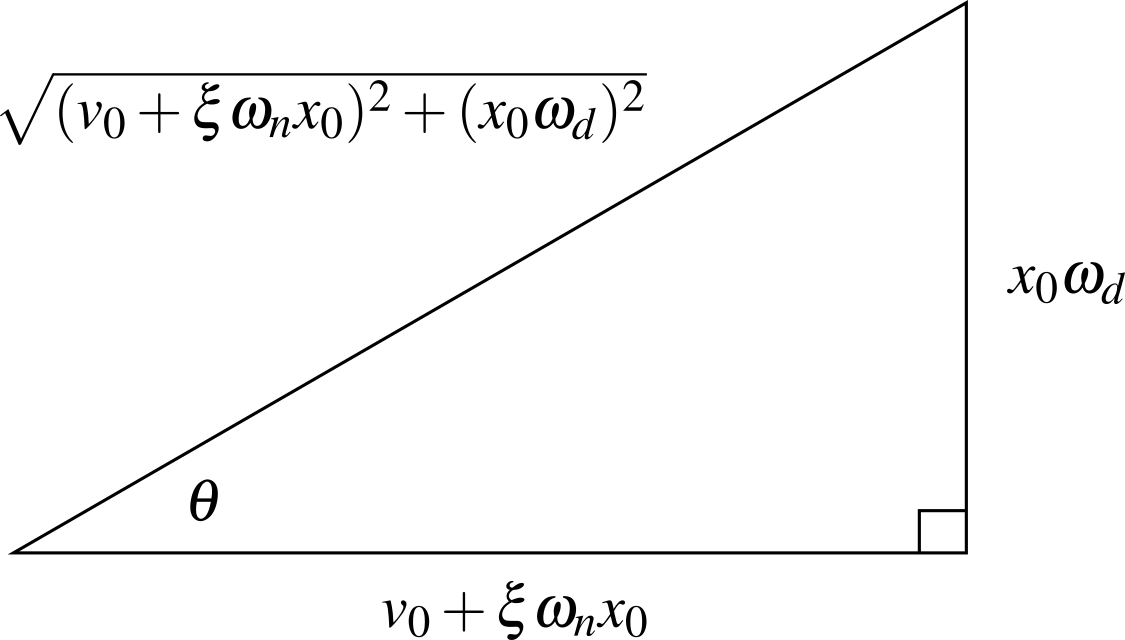
\includegraphics[width=0.4\textwidth]{../../Figures/Trigonometric_relationship_underdamped.png}
			\end{figure}
			we get: 
			\begin{equation}
				\text{sin}(\phi) = \frac{x_0\omega_d}{\sqrt{(v_0+\zeta\omega_nx_0)^2 + (x_0\omega_d)^2}}
			\end{equation} 	
			and applying $A=x_0/\text{sin}(\phi)$ we get:
			\begin{equation}
				A = \frac{\sqrt{(v_0+\zeta\omega_nx_0)^2 + (x_0\omega_d)^2}}{\omega_d} = \sqrt{x_0^2 + \Bigg( \frac{v_0 + \zeta \omega_n x_0}{\omega_d}\Bigg)^2}
			\end{equation} 								
			Finally, collecting all of our important equations:
			\begin{itemize}
			\item Critical damping coefficient: $c_{\text{cr}} = 2\sqrt{km} = 2m\omega_n$
			\item Damping ratio: $	\zeta = \frac{c}{c_{\text{cr}}} = \frac{c}{2\sqrt{km}} = \frac{c}{2m\omega_n}$
			\item Damped natural frequency: $\omega_d = \omega_n\sqrt{1-\zeta^2}$
			\item Solution for underdamped system: $x(t) = Ae^{-\zeta\omega_nt}\text{sin}(\omega_dt + \phi)$, where: \begin{align*}
						A = \frac{\sqrt{(v_0+\zeta\omega_nx_0)^2 + (x_0\omega_d)^2}}{\omega_d} & \hspace{1.5cm} \phi = \text{tan}^-1\Bigg(\frac{x_0\omega_d}{v_0+\zeta\omega_nx_0}\Bigg) 
						\end{align*}
			\end{itemize}

		\subsection*{Over damped motion}
			
			In the case of overdamped systems, $1<\zeta$, the solutions for $\lambda$ are distinct real roots that are written as:
			\begin{equation}
				\lambda_{1} = -\zeta\omega_n - \omega_n \sqrt{\zeta^2-1}
			\end{equation} 			
			and:
			\begin{equation}
				\lambda_{2} = -\zeta\omega_n + \omega_n \sqrt{\zeta^2-1}
			\end{equation} 
			The solution for the EOM using the assumed solution then becomes:
			\begin{equation}
				x(t) = e^{-\zeta\omega_nt}(a_1e^{-\omega_n \sqrt{\zeta^2-1}t} + a_2e^{+\omega_n \sqrt{\zeta^2-1}t}) 
			\end{equation}
			This equation represents a non-oscillating response of the system. Again, $a_1$ and $a_2$ are solved for using known boundary conditions $x_0$ and $v_0$ such that:
			\begin{align}
				a_1 &= \frac{-v_0+\Big(-\zeta+\sqrt{\zeta^2-1}\Big)\omega_n x_0}{2\omega_n\sqrt{\zeta^2-1}} \\ 
				a_2 &= \frac{v_0+\Big(\zeta+\sqrt{\zeta^2-1}\Big)\omega_n x_0}{2\omega_n\sqrt{\zeta^2-1}}
			\end{align}				
			Typical responses for a overdamped system with various initial conditions are shown below:
			\begin{figure}[H]
				\centering
				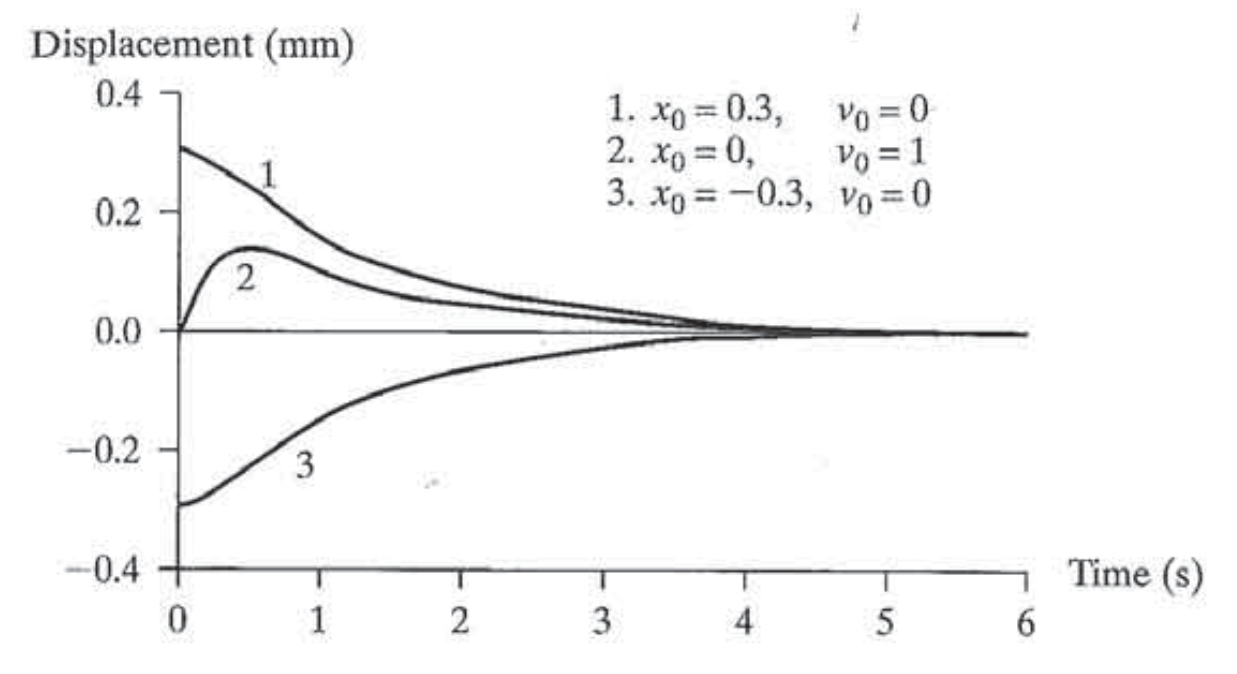
\includegraphics[width=0.6\textwidth]{../../Figures/Overdamped_system.png}
			\end{figure}
			
		\subsection*{Critically damped motion}
			
			In the case of critically damped systems, $\zeta=1$, the solutions for $\lambda$ will be equal negative real numbers, therefore from before:
			\begin{equation}
				\lambda_{1,2} = -\zeta\omega_n \pm \omega_n \sqrt{\zeta^2-1}
			\end{equation}
			We get:
			\begin{equation}
				\lambda_{1} = \lambda_{2} = -\omega_n
			\end{equation} 			
			Because both solutions ($a_1$ and $a_2$) are the same, we multiply the second solution by $t$ so the solution for a critically damped system is in the same form as before. The solution for the EOM using the assumed solution then becomes:
			\begin{equation}
				x(t) = a_1e^{-\omega_nt} + a_2te^{-\omega_nt} 
			\end{equation} 
			This simplifies into:			
			\begin{equation}
				x(t) = (a_1+a_2t) e^{-\omega_nt} 
			\end{equation}
			This equation represents a non-oscillating response of the system. Again, $a_1$ and $a_2$ are solved for using known boundary conditions $x_0$ and $v_0$ such that:
			\begin{align}
				a_1 &= x_0 \\ 
				a_2 &= v_0+\omega_nx_0
			\end{align}				
			Typical responses for a overdamped system with various initial conditions are shown below:
			\begin{figure}[H]
				\centering
				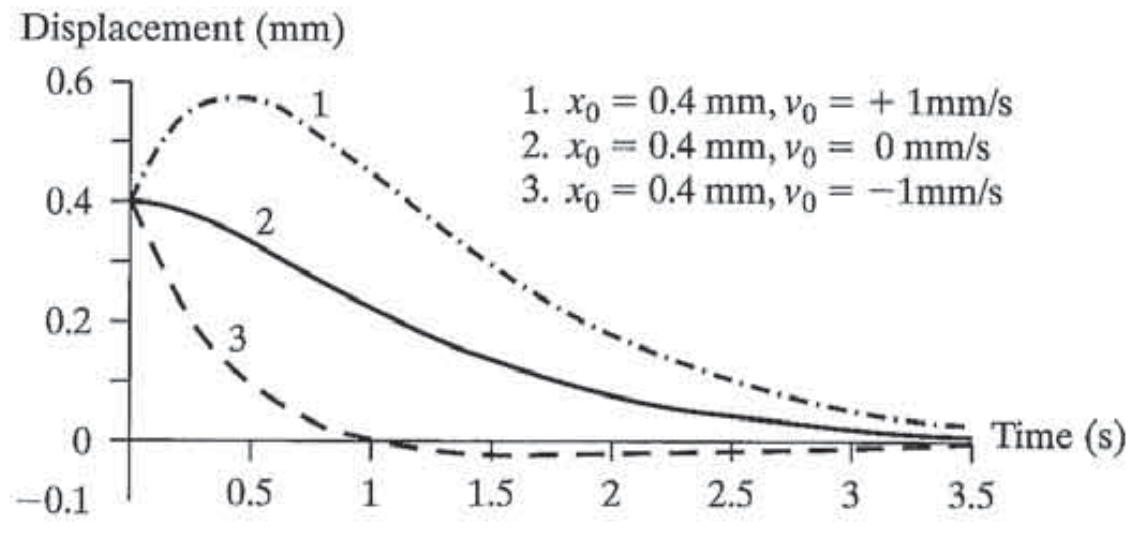
\includegraphics[width=0.6\textwidth]{../../Figures/Critically_damped_system.png}
			\end{figure}

		\subsection*{Standard Form of the EOM}
			Typically, we write the EOM:
			\begin{equation}
				m\ddot{x}(t) + c \dot{x}(t) + kx(t) = 0
			\end{equation}
			In what is known as standard form. First, every term is divided by $m$ such that:
			\begin{equation}
				\ddot{x}(t) + \frac{c}{m}\dot{x}(t) + \frac{k}{m}x(t) = 0
			\end{equation}		
			This can be rearranged to the \textbf{standard form}:
			\begin{equation}
				\ddot{x}(t) + 2\zeta\omega_n\dot{x}(t) + \omega_n^2x(t) = 0
			\end{equation}	
		\subsection*{Important items from today}
	
			\begin{itemize}
				\item There are three types of damping cases, under, critical, and over. 
				\item The under damped system is the only one that oscillates, and as such is of the most importance to this class. 
			\end{itemize}

			\begin{table}[h!]
				\centering
				\begin{tabular}{lccc}
					\toprule
					damping case & critical damping ratio & radicand & solutions  \\ \midrule
					under damped &  $0<\zeta<1$ & $c^2-4km<0$ & complex conjugate pairs \\
					critically damped & $\zeta=1$ & $c^2-4km=0$ & equal negative real numbers \\
					over damped & $1<\zeta$  & $c^2-4km>0$ & distinct negative real numbers \\ \bottomrule
				\end{tabular}
			\end{table}
			
			\subsection*{Example 1}	Consider the following 1-DOF system, where $k = 857.8$ N/m, $c=7.8$ kg/s, and $m=49.2\times10^{-3}$ kg, calculate the damped frequency in rad/s and Hz. What damping case is this system?  	
			\begin{figure}[H]
				\centering
				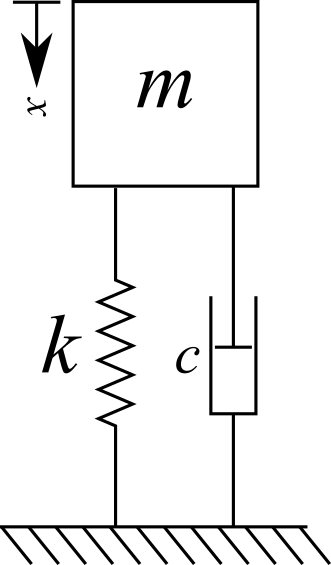
\includegraphics[width=0.13\textwidth]{../../Figures/1-damped_DOF-mass_vertical.png}
			\end{figure}		

			\subsection*{Example 1} Calculate the undamped frequency:
			\begin{equation}
				\omega_n = \sqrt{\frac{k}{m}}= \sqrt{\frac{857.8}{49.2\times10^{-3}}} = 132 \hspace{1ex}\text{rad/s}
			\end{equation}	
			The systems critical damping value:
			\begin{equation}
				c_{\text{cr}} = 2\sqrt{km}= 2\sqrt{k = 857.8 \cdot 49.2\times10^{-3}} = 12.993 \hspace{1ex}\text{kg/s}
			\end{equation}		
			And the critical damping ratio:
			\begin{equation}
				\zeta = \frac{c}{c_{\text{cr}}} = \frac{7.8}{12.993} = 0.600
			\end{equation}				
			This can also be expressed as 60\% damped, this is a underdamped system, and the system will oscillate. Now we can calculate the damped frequency:
			\begin{equation}
				\omega_d = \omega_n\sqrt{1-\zeta^2} = \omega_n\sqrt{1-0.600^2} = 105.6 \hspace{1ex}\text{rad/s}
			\end{equation}		
			Therefore, the system oscillates at 105.6 rad/sec or 16.81 Hz

		\subsection*{Example 2} 
			For a damped one DOF system where $m$, $c$, and $k$ are known to be $m$ = 1 kg, $c$ = 2 kg/s, and $k$ = 10 N/m. Calculate the value of $\zeta$ and $\omega_n$. Is the system overdamped, underdamped, or critically damped?	
			
			The natural frequency is calculated as
			\begin{equation}
				\omega_n = \sqrt{\frac{k}{m}} = \sqrt{\frac{10}{1}} = 3.16 \hspace{1ex} \text{rad/s}
			\end{equation}
			The damping can be calculated as:
			\begin{equation}
				\zeta = \frac{c}{2\omega_n m} = \frac{2}{2\Big(\sqrt{\frac{10}{1}}\Big)(1)} = \frac{1}{\sqrt{10}} = 0.316 \hspace{1ex} \text{rad/s}
			\end{equation}
			So the damped natural frequency is equal to:
			\begin{equation}
				\omega_d = \omega_n\sqrt{1-\zeta^2} =  \sqrt{10}\sqrt{1-\bigg(\frac{1}{\sqrt{10}}\bigg)^2} = 0.3 \hspace{1ex} \text{rad/s}
			\end{equation}			
			As $0<\zeta<1$ the system is underdamped. 			

		\subsection*{Example 3} 
			For the following industrial device consisting of a mass isolated from its fixtures by rubber dampers provide an estimate of the systems oscillating frequency.		
			\begin{figure}[H]
				\centering
				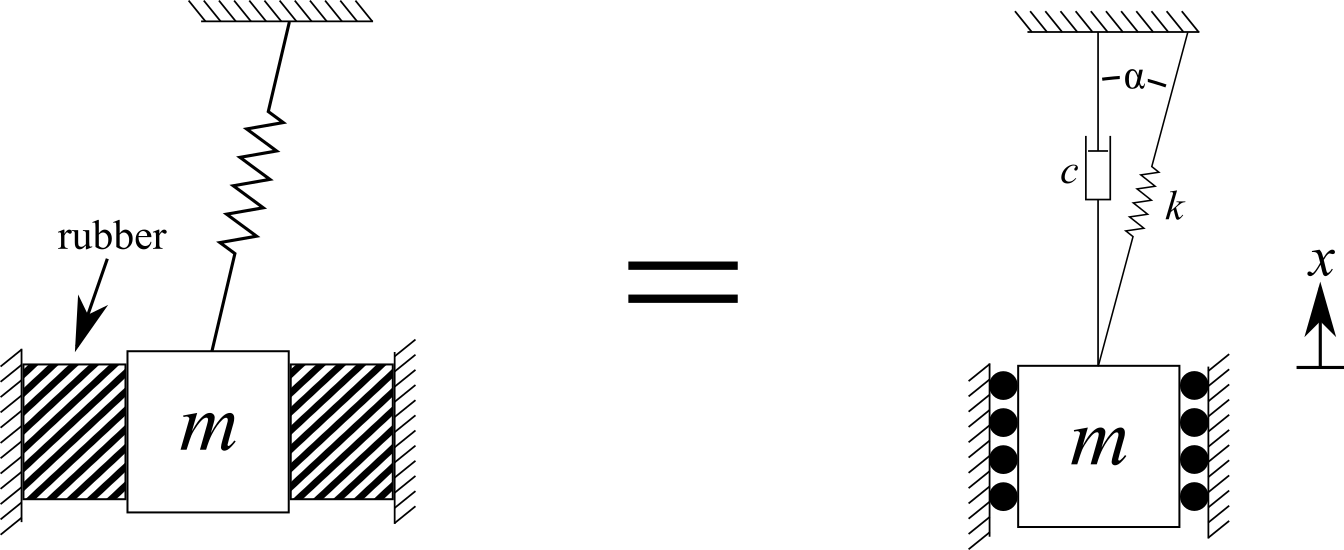
\includegraphics[width=0.6\textwidth]{../../Figures/rubber_mounted_mass.png}
			\end{figure}
			As we only want an estimate of the frequency, we can assume the displacement is small and as such $\alpha$ of the displaced mass is equal $\alpha$ of the resting mass. This leads to the FBD for the resting and displaced masses.
			\begin{figure}[H]
				\centering
				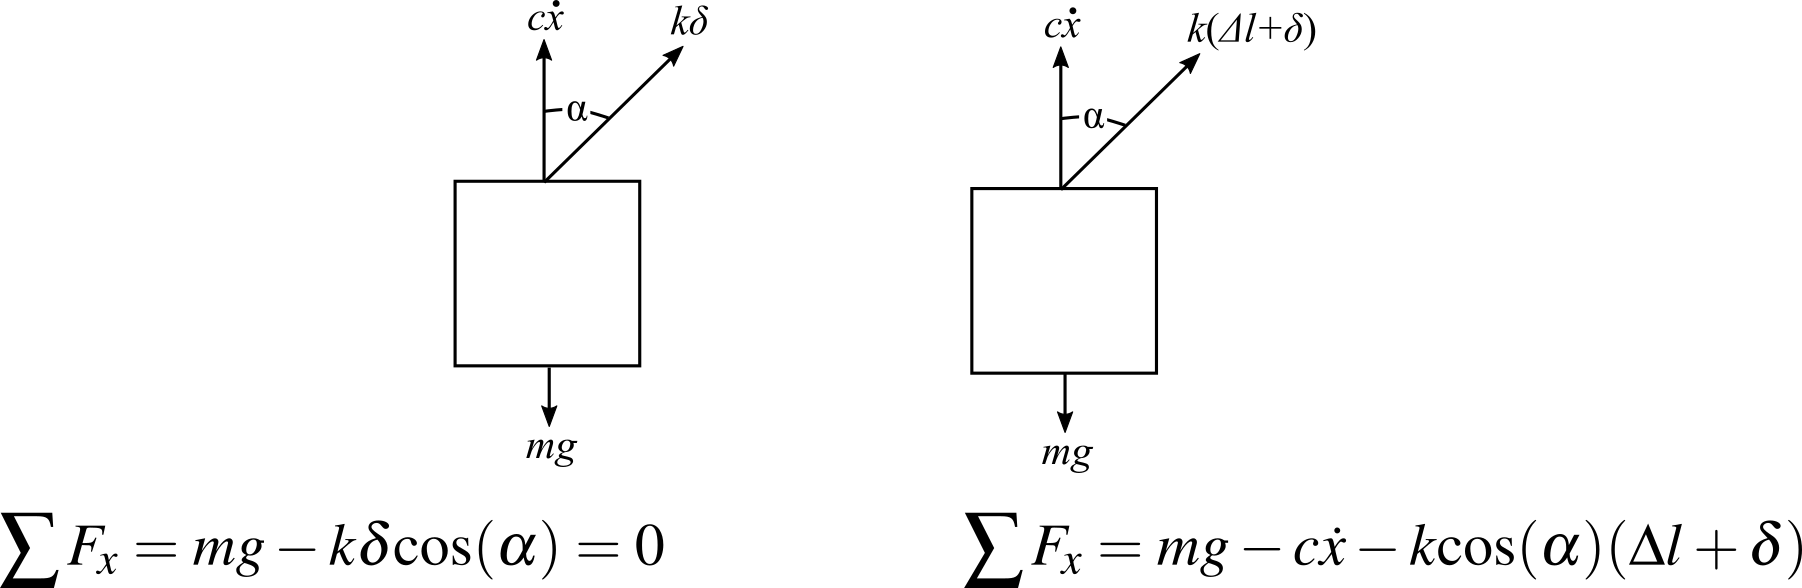
\includegraphics[width=0.9\textwidth]{../../Figures/rubber_mounted_mass_FBD.png}
			\end{figure}
%			\begin{equation}
%				\sum F_x = mg -k\delta\text{cos}(\alpha) =0
%			\end{equation}				
%			\begin{equation}
%				\sum F_x = mg - c\dot{x}-k\text{cos}(\alpha)(\Delta l+\delta)
%			\end{equation}					
			Applying newtons second law and combining these equations yields:
			\begin{equation}
				m\ddot{x} + c\dot{x} + k \Delta l \text{cos}(\alpha) =0
			\end{equation}			
			As we assumed the displacement is small and $\alpha$ remains unchanged, the assumption that cos($\alpha$) = $h/l$ is equivalent to cos($\alpha$) = $x/\Delta l$ is logical (draw out the triangles if needed), therefore the prior equation becomes: 
			\begin{equation}
				m\ddot{x} + c\dot{x} + k \Delta l \frac{x}{\Delta l} =m\ddot{x} + c\dot{x} + k x  = 0
			\end{equation}	
			as $\alpha$ and $x$ are small. Therefore, the frequency can be estimated as:		
			\begin{equation}
				\omega_d = \omega_n\sqrt{1-\zeta^2}
			\end{equation}
			once the values for the system are known or measured. 			
			
											 
%\subsection*{How can we solve this new ODE?}
%
%Again, we build the equation based on observations of a system, 
%
%\begin{equation}
%{x}(t) = A\text{sin}(\omega_n t + \phi)
%\end{equation}
%
%Take the derivative to get velocity:
%
%\begin{equation}
%\dot{x}(t) = A\omega_n\text{cos}(\omega_n t + \phi)
%\end{equation}
%
%Take the derivative again to get acceleration:
%
%\begin{equation}
%\ddot{x}(t) = -A\omega_n^2\text{sin}(\omega_n t + \phi)
%\end{equation}
%
%Our ODE now becomes:
%
%\begin{equation}
%m\big(-A\omega_n^2\text{sin}(\omega_n t + \phi)\big) + c\big(A\omega_n\text{cos}(\omega_n t + \phi)\big) + k\big(A\omega_n\text{sin}(\omega_n t + \phi)\big) = 0
%\end{equation}
%
%If we divide both sides by $A\text{sin}(\omega_n t + \phi)$ we are left with:
%\begin{equation}
%-m\omega_n^2+k = 0
%\end{equation}
%
%
%We can solve an ODE by observing a system, for a location $x$, at a time $t$; $x(t)$. This system is called ``simple harmonic motion'':
%\begin{itemize}
%	\item System oscillates $\rightarrow$ use a sin function to model this 
%	\item System oscillates at different speed $\rightarrow$ use a parameter to to adjust $\omega_n$ in rad/s.
%	\item System has different starting points $\rightarrow$ use a parameter to to adjust $\phi$ in rad.
%	\item Systems have different amplitudes $\rightarrow$ use a parameter to to adjust $A$ in meters.
%\end{itemize}
%
%\begin{figure}[H]
%	\centering
%	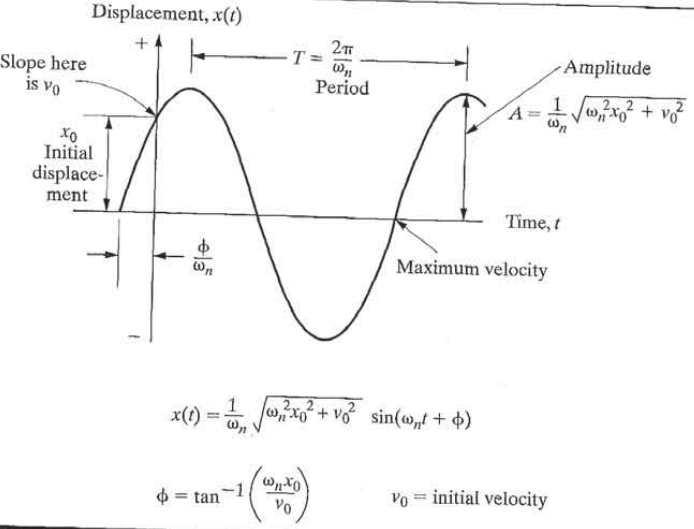
\includegraphics[width=0.8\textwidth]{../../Figures/simple_harmonic_motion.png}
%\end{figure}
%
%Now we build the equation we have just proposed, 
%
%\begin{equation}
%{x}(t) = A\text{sin}(\omega_n t + \phi)
%\end{equation}
%
%Take the derivative to get velocity:
%
%\begin{equation}
%\dot{x}(t) = A\omega_n\text{cos}(\omega_n t + \phi)
%\end{equation}
%
%Take the derivative again to get acceleration:
%
%\begin{equation}
%\ddot{x}(t) = -A\omega_n^2\text{sin}(\omega_n t + \phi)
%\end{equation}
%
%Our ODE now becomes:
%
%\begin{equation}
%m\big(-A\omega_n^2\text{sin}(\omega_n t + \phi)\big) + k\big(A\omega_n\text{cos}(\omega_n t + \phi)\big) = 0
%\end{equation}
%
%Is this true? If we divide both sides by $A\text{sin}(\omega_n t + \phi)$ we are left with:
%\begin{equation}
%-m\omega_n^2+k = 0
%\end{equation}
%
%rearranged into the standard form:
%
%\begin{equation}
%\omega_n= \sqrt{\frac{k}{m}}
%\end{equation}
%
%This is not an ODE so the equation is solvable and testable. This is the first important equation and relates the frequency of a system to stiffness and mass. This equation leads to:
%
%
%\begin{equation}
%T= \frac{2 \pi}{\omega_n}
%\end{equation}
%
%
%\begin{equation}
%f_n= \frac{\omega_n}{2 \pi}
%\end{equation}
%
%
%
%
%
%
%\subsection*{solve for $A$ and $\phi$}
%Now we need to solve for $A$ and $\phi$. The ODE was a second order so we need two constants ($A$ and $\phi$) to solve it, both of these can be determined by its initial state ($x=0$). 
%
%\begin{equation}
%{x}(0) = A\text{sin}(\omega_n 0 + \phi) = A\text{sin}(\phi) 
%\end{equation}
%\begin{equation}
%\dot{x}(0) = A\omega_n\text{cos}(\omega_n0 + \phi) = A\omega_n\text{cos}(\phi)
%\end{equation}
%
%We can solve for $A$ and $\phi$ using these two equations. For $\phi$:
%
%
%\begin{equation}
%A = \frac{x_0}{\text{sin}(\phi) }
%\end{equation}
%and:
%\begin{equation}
%A = \frac{v_0}{\omega_n\text{cos}(\phi)}
%\end{equation}
%therefore:
%\begin{equation}
%\frac{x_0 \omega_n}{\text{sin}(\phi)} = \frac{v_0}{\text{cos}(\phi)} 
%\end{equation}
%and:
%\begin{equation}
%\frac{x_0\omega_n}{v_0} = \frac{\text{sin}(\phi)}{\text{cos}(\phi)}
%\end{equation}
%finally:
%\begin{equation}
%\phi = \text{tan}^{-1}\bigg(\frac{x_0\omega_n}{v_0}\bigg)
%\end{equation}
%
%Now we can solve for $A$, in the same manner:
%
%
%\begin{equation}
%\text{sin}(\phi) = \frac{x_0}{A}
%\end{equation}
%and:
%\begin{equation}
%\text{cos}(\phi) = \frac{v_0}{\omega_nA}
%\end{equation}
%knowing that $\text{sin}(\phi)^2+\text{cos}(\phi)^2=1$ and applying $\frac{\omega_n}{\omega_n}$:
%\begin{equation}
%\bigg(\frac{\omega_n}{\omega_n}\bigg)^2\bigg(\frac{x_0}{A}\bigg)^2  = \bigg(\frac{v_0}{\omega_nA}\bigg)^2
%\end{equation}
%Which becomes:
%\begin{equation}
%\omega_n^2x_0^2+v_0^2=A^2\omega_n^2 
%\end{equation}
%rearranges to:
%
%\begin{equation}
%A = \sqrt{\frac{\omega_n^2x_0^2+v_0^2}{\omega_n}}
%\end{equation}
%
%\section*{Now we can get the response for simple harmonic motion}
%
%Using our equation for ${x}(t) = A\text{sin}(\omega_n t + \phi)$, we get:
%
%\begin{equation}
%{x}(t) = \sqrt{\frac{\omega_n^2x_0^2+v_0^2}{\omega_n}}\text{sin}\Bigg(\omega_n t + \bigg( \text{tan}^{-1}\bigg(\frac{x_0\omega_n}{v_0}\bigg)\bigg)\Bigg)
%\end{equation}
%
%\begin{itemize}
%	\item This is the free response of the system because no input is applied after t=0
%	\item This is simple harmonic motion, later on we will discusses forced harmonic excitation.
%\end{itemize}
%
%\section*{Important items from today}
%
%\begin{itemize}
%	\item EOM is a 2nd order DOE we solved with {x}(t) = \begin{equation}
%	{x}(t) = A\text{sin}(\omega_n t + \phi)
%	\end{equation} and \begin{equation}
%	\omega_n= \sqrt{\frac{k}{m}}
%	\end{equation}
%	\item A mathematical model for the displacement for a simple harmonic motion is. \begin{equation}
%	{x}(t) = \sqrt{\frac{\omega_n^2x_0^2+v_0^2}{\omega_n}}\text{sin}\Bigg(\omega_n t + \bigg( \text{tan}^{-1}\bigg(\frac{x_0\omega_n}{v_0}\bigg)\bigg)\Bigg)
%	\end{equation}
%\end{itemize}
%








\end{document}